\documentclass{hw}

\title{Assignment 0}
\author{MATH 168, Spring 2022}
\date{Due Monday, April 4th}

\begin{document}


\section*{Assignment 0}

This is the first assignment of MATH 168. 
It has three primary purposes: 
\begin{itemize}
    \item To help you re-engage with some important ideas and results from the two mathematical foundations of the study of networks: linear algebra and probability. 
    \item To get you ``set up'' for the course by installing software for network computations and introducing yourself to the class on Campuswire. 
    \item To get you used to how the homework system works in MATH 168, as it's a bit different from what you may be used to. 
\end{itemize}
This assignment should be submitted on Gradescope, with pages assigned to each problem.  
Writing your solutions in \LaTeX{} is highly encouraged but not required. 

\subsection*{Specifications Grading}

Before starting on this assignment, it's a good idea to consult the \href{https://www.philchodrow.com/intro-networks/syllabus/syllabus.html#homework-assignments}{syllabus}. 
Here are the key points that you should keep in mind when working on this assignment.
\begin{itemize}
    \item There is no partial credit on homework problems. You receive credit for a problem by completing the entire problem (including all parts, if applicable), to a high standard of correctness and communication. 
    This standard is enumerated by \emph{specifications}. 
    \item You will have \textbf{multiple attempts} to complete each problem. 
    After the initial submission by the first due date, your assignment will be assessed. 
    Problems that meet specifications will receive credit. 
    If you've attempted some problems but not met specifications, you can revise your solutions and resubmit them. 
    If they now meet specs, you get credit! 
    \item If you submitted a problem by the deadline with less than 50\% of the problem completed, as determined by the TA, then you can resubmit for 50\% credit. 
    This policy is here to incentivize you to do your best on the problems by the stated deadline, which keeps you on track and keeps our TA's workload manageable. 
    \item You don't actually have to do all homework problems assigned: you have the equivalent of 5 homework problem drops throughout the quarter. 
    It's still a good idea to attempt all problems though, as this will allow you to make up for, say, a rough day on the midterm exam. 
    The syllabus has details on how your final grade will be calculated. 
\end{itemize}

\pagebreak

\subsection*{Specifications}

This is the list of specifications that you should meet for most problems in order to receive credit. 
These specifications apply to all problems that request you to write a \textbf{proof} or \textbf{argument} for a mathematical statement. 

You can think of this like a checklist: if, for a given problem, you can check of each item, then you should expect to receive credit! 
Going down this checklist is exactly what the TA will do to grade your work. 

Please remember that \textbf{these specifications apply to every part of a problem}. 
To receive credit on a problem with parts (a), (b), and (c), you need to meet the specifications on all three parts.  

\subsubsection*{Correctness}

\begin{itemize}
    \item Each direction in the problem statement is followed. 
    \begin{itemize}
        \item \emph{Note}: You are required to follow only \emph{directions}, not \emph{hints}. 
        That said, I include the hints with the intention of making your life easier! 
    \end{itemize}
    \item The overall structure is mathematically sound and supports the required result. 
\end{itemize}

\subsubsection*{Exposition}

\begin{itemize}
    \item Each step is carefully justified in terms of results from the course, results from the course text, or results from previous courses. 
    \item The proof or argument is presented using clear and engaging English prose. 
    The proof or argument is written in English sentences. 
    There is at least as much English text as there are mathematical symbols. 
    Grammar and spelling errors are acceptable provided that the meaning is clear. 
\end{itemize}

\subsubsection*{Other}

We'll also see problems in which you are expected to write some code, show a plot, write a brief reflection, or perform some other task. 
In this case, the specifications will be included with the problem statement. 


\problem{}
    Join the class Campuswire forum if you haven't already! 
    I've invited all of you, but if you didn't receive the invitation, please contact me. 

    Write a post on Campuswire in which you briefly respond to the following questions: 
    \begin{enumerate}
        \item Who are you? Let us know: 
        \begin{itemize}
            \item Your name, and, if you choose, your pronouns. 
            \item Your major area of study. 
            \item A fun fact about yourself. 
        \end{itemize}
        \item Why are you interested in learning about networks? 
        \item What is one question you have about the role that networks play in your life today?
        \item What is something related to networks that you might like to create or investigate by the end of the quarter? 
    \end{enumerate}

    Then, look for at least two other posts by classmates whose answer to (iii) sounds interesting to you. 
    Reply with a friendly greeting and a few sentences describing the overlap in your interests. 

    \textbf{Take screencaps} of your post and your reply to your classmates' posts (3 screencaps total). Include them with your file submission on Gradescope, and tag them with this problem number when assigning pages.  


\problem{}

You're likely familiar with the algebraic definition of the eigenvalues and eigenvectors of a matrix $\mathbf{A}$ as solutions to the equation $\mathbf{A}\mathbf{v} = \lambda \mathbf{v}$. 
In this problem, we will prove an additional viewpoint on eigenvalues and eigenvectors that is especially important in network science and many other fields of applied mathematics: 
\begin{quote}
    \emph{For symmetric matrices, eigenpairs are solutions of optimization problems.} 
\end{quote}
Let $\lVert\mathbf{v} \rVert$ be the Euclidean norm of a vector $\mathbf{v}$. 
Here's our theorem: 
\begin{thm}\label{thm:variational}
    Let $\mathbf{A} \in \mathbb{R}^{n\times n}$ be a symmetric matrix. 
    Let $\lambda_1,\ldots,\lambda_n$ be the eigenvalues of $\mathbf{A}$ ordered from smallest ($\lambda_1$) to largest ($\lambda_n$).  
    Then, 
    \begin{align*}
        \lambda_n = \max_{\mathbf{v} \in \mathbb{R}^n} \left\{\mathbf{v}^T\mathbf{A}\mathbf{v} \;\big|\; \lVert{\mathbf{v}}\rVert = 1\right\} \;.
    \end{align*}
\end{thm}
In words, the largest value of the function $f(\mathbf{v}) = \mathbf{v}^T\mathbf{A}\mathbf{v}$ that can be obtained by picking a vector $\mathbf{v} \in \mathbb{R}^n$ satisfying $\lVert \mathbf{v} \rVert = 1$ is $\lambda_n$. 
The reason that \Cref{thm:variational} matters from an applied standpoint is that many network science and data analysis tasks correspond to maximizing functions that look like $f(\mathbf{v}) = \mathbf{v}^T\mathbf{A}\mathbf{v}$.  


\part

    Prove \Cref{thm:variational} in three steps. 
    \begin{enumerate}
        \item Expand $\mathbf{A}$ in an orthonormal basis of eigenvectors: 
        \begin{align*}
            \mathbf{A} = \sum_{i = 1}^n \lambda_i\mathbf{u}_i\mathbf{u}_i^T\;,
        \end{align*}
        where each $\mathbf{u}_i$ is an eigenvector $\mathbf{A}$ with eigenvalue $\lambda_i$. 
        As a reminder, orthonormality means that $\lVert \mathbf{u}_i \rVert = 1$ and $\mathbf{u}_i^T \mathbf{u}_j = 1$ if $i = j$ and $0$ otherwise.   
        Explain carefully why you are allowed to perform this expansion (cite a theorem). 
        \item Write $\mathbf{v} = \sum_{i = 1}^n \alpha_i \mathbf{u}_i$ for some undetermined coefficients $\{\alpha_i\}$, and explain why you are allowed to do this. 
        Compute $\lVert \mathbf{v}\rVert$ in terms of the coefficients $\{\alpha_i\}$, and determine what the constraint $\lVert \mathbf{v} \rVert = 1$ implies about $\{\alpha_i\}$. 
        \item Finally, use the first two steps to compute $\mathbf{v}^T\mathbf{A}\mathbf{v}$ directly in terms of $\{\lambda_i\}$ and $\{\alpha_i\}$. 
        Show that the result is maximized when $\alpha_n = 1$ and $\alpha_i = 0$ for $i < n$. 
        Include a closing sentence to help your reader connect this final result to \Cref{thm:variational}. 
    \end{enumerate}
    
    

\part 

    Prove \Cref{thm:variational} (again) using the \emph{principle of Lagrange multipliers}. 
    The principle of Lagrange multipliers states that, if $\mathbf{x}$ solves the problem 
    \begin{align*}
        \max_{\mathbf{x} \in \mathbb{R}^n} \left\{f(\mathbf{x}) \;\big|\; g(\mathbf{x}) = 0\right\} \;,
    \end{align*}
    then $\mathbf{x}$ must also satisfy the equation 
    \begin{align*}
        \nabla f(\mathbf{x}) + c \nabla g(\mathbf{x}) = 0
    \end{align*}
    for some scalar $c \in \mathbb{R}$, provided that $f$ and $g$ satisfy certain technical conditions (which you may assume are satisfied here). 
    
    You may assume without proof that any continuous function on the unit sphere $S^{n-1} = \{\mathbf{v} : \lVert \mathbf{v}\rVert = 1\}$ possesses at least one maximum value (this follows from the compactness of $S^{n-1}$). 
    You may also assume without proof that the function $f(\mathbf{v}) = \mathbf{v}^T\mathbf{A}\mathbf{v}$ is continuous. 
    State clearly where you use these facts in your proof. 
    Please again make sure to explicitly state where you use the hypothesis that $\mathbf{A}$ is symmetric. 

    \begin{hint}
        $\lVert \mathbf{v} \rVert =1$ if and only if $\lVert \mathbf{v} \rVert^2 =1$. 
        One of these expressions will be easier to differentiate than the other one. 
    \end{hint}

    

    \part 
    
    Using \Cref{thm:variational}, give an \emph{extremely short} proof that
    \begin{align*}
        \lambda_1 = \min_{\mathbf{v} \in \mathbb{R}^n} \left\{\mathbf{v}^T\mathbf{A}\mathbf{v} \;\big|\; \lVert{\mathbf{v}}\rVert = 1\right\} \;.
    \end{align*} 

    \part 

    Suppose that $\mathbf{u}_n$ is an eigenvector of $\mathbf{A}$ with eigenvalue $\lambda_n$. 
    Prove that 
    \begin{align*}
        \lambda_{n-1} = \max_{\mathbf{v} \in \mathbb{R}^n} \left\{\mathbf{v}^T\mathbf{A}\mathbf{v} \;\big|\; \lVert{\mathbf{v}}\rVert = 1\;, \; \mathbf{v}^T\mathbf{u}_n = 0\right\}\;. 
    \end{align*}
    \emph{Hint}: This is a very short proof if you use one of the previous parts, although not quite as short as Part (c). 
    

     

\problem{(Stationary Distributions of Markov Chains)}



    A finite-state, discrete-time \emph{ Markov chain} is a sequence of random variables $X_1,X_2,\ldots,X_t,\ldots$ such that: 

    \begin{itemize}
        \item Each $X_t$ takes values in some finite set $\mathcal{X}$ of size $n$ called the \emph{state space} of the chain. 
        \item The sequence satisfies the \emph{Markov property}: for any states $x, y_1,y_2,\ldots \in \mathcal{X}$, it holds that 
        \begin{align*}
            \mathbb{P}(X_{t+1} = x | X_t = y_t, X_{t-1} = y_{t-1},\ldots,X_1 = y_1) = \mathbb{P}(X_{t+1} = x | X_t = y_t)\;.
        \end{align*}
        If we think of time $t$ as being ``right now,'' the Markov property states that ``the future'' state $X_{t+1}$ depends only on ``the present'' $X_t$, and not on ``the past'', which includes all the variables $X_{t-1},X_{t-2},\ldots,X_1$. 

    A finite-state, discrete-time Markov chain is fully specified by the initial state $X_1$ and the set of \emph{transition probabilities} of the form $\mathbb{P}(X_{t+1} = j | X_t = i)$. 
    \end{itemize}

    \part 

    
    

    Let $\mathbf{A} \in \mathbb{R}^{n\times n}$ have nonnegative entries. 
    Prove that $\mathbf{A}$ has a left eigenvector with nonnegative entries. 

    
    \begin{hint}
    A famous fixed-point theorem of topology (which you may use without proof) states that, if $S$ is a compact and convex set, then any continuous function $f:S\rightarrow S$ must have a \emph{fixed point}; i.e. a point $s \in S$ such that $f(s) = s$.  
    
    The set 
    \begin{align*}
        \mathcal{P} = \left\{\mathbf{v} \in \mathbb{R}^{n} : v_i \geq 0\;,  \sum_{i=1}^{n} v_i = 1\right\}\;,
    \end{align*}
    often called the \emph{probability $n-1$-simplex}, is compact and convex (so, you can apply the fixed point theorem even if you don't know or remember what ``compact'' and ``convex'' mean). 
    Can you use $\mathbf{A}$ to construct a continuous function $f:\mathcal{P} \rightarrow \mathcal{P}$ such that a fixed point of $f$ satisfies an eigenvector relation for $\mathbf{A}$?
    \end{hint}


    \part

    Let $\mathbf{q} \in \mathcal{P}$. 
    Construct a matrix $\mathbf{P}$ such that, if $\mathbb{P}(X_{t} = i) = q_i$, then $\mathbb{P}(X_{t+1} = j) = [\mathbf{q}^T\mathbf{P}]_j$. 

    \begin{hint}
        Compute $\mathbb{P}(X_{t+1} = j)$ using the law of total probability, conditioning on the prior state $X_t$. 
        You can treat the transition probabilities as known data and use them when constructing $\mathbf{P}$. 
    \end{hint}

    

    \part 

    Prove that $\mathbf{P}$ has a left eigenvector $\pi\in \mathcal{P}$ with eigenvalue $1$. 
    That is $\pi^T\mathbf{P} = \pi^T$. 

    \begin{hint}
    First, use Part (a) to argue that $\mathbf{P}$ has a left eigenvector with nonnegative entries. 
    Second, argue that you can take this eigenvector to be an element of $\mathcal{P}$, and call the result $\pi$.  
    Finally, add up the components on both sides of the eigenvector relation $\pi^T\mathbf{P} = \lambda \pi^T$ to show that $\lambda = 1$. 
    \end{hint}

    \part 

    Consider a Markov chain in which $X_1$ is distributed according to $\pi$. 
    What is the distribution of $X_{2022}$? 


    \subsubsection{Note}

    The distribution vector $\pi$ is often called a \emph{stationary distribution} of the Markov chain. 
    Under mild additional assumptions, it is possible to prove that $\pi$ is the unique stationary distribution associated to the Markov process, and that the distribution of $X_t$ converges to $\pi$ as $t$ grows large. 


% \problem{}

    

%     Let $X_1,X_2\ldots,$ be an infinite sequence of i.i.d. random variables. 
%     Let $N$ be a strictly positive random variable that is independent of the sequence $\{X_1,X_2,\ldots\}$. 
%     Let 
%     \begin{align*}
%         Y = \sum_{i = 1}^N X_i\;. 
%     \end{align*}
%     Prove that $\mathbb{E}[Y] = \mathbb{E}[X_1]\mathbb{E}[N]$. 


\problem{}

Install some software for computing with networks. 
If you don't have a strong preference, I recommend that you use Python and the NetworkX package, as this is what we'll be primarily using for demonstrations and support. 
You're allowed to use other tools (R, Julia, Matlab) if you choose, but please know that we may not be able to help you much on these. 

The easiest way to install Python and NetworkX for someone who hasn't used them before is to download \href{https://www.anaconda.com}{Anaconda}, which includes NetworkX built in. 
You can then start Anaconda and open a Jupyter Notebook in which to write and run code. 
Note: if you've previously installed Anaconda, it's recommended to uninstall and reinstall it. 
I encountered some errors with NetworkX that went away after a clean reinstallation. 

Open your software of choice. Write code to do two things: 
\begin{itemize}
    \item Produce a visualization of a simple network. 
    \item Print your name. 
\end{itemize}
Take a screencap of your code and output, including both your network and your name. 
Submit this screencap on Gradescope. 

Here is an example solution using Python and NetworkX. 
Copying and running this code exactly (while modifying your name) is sufficient to receive full credit on this problem. 

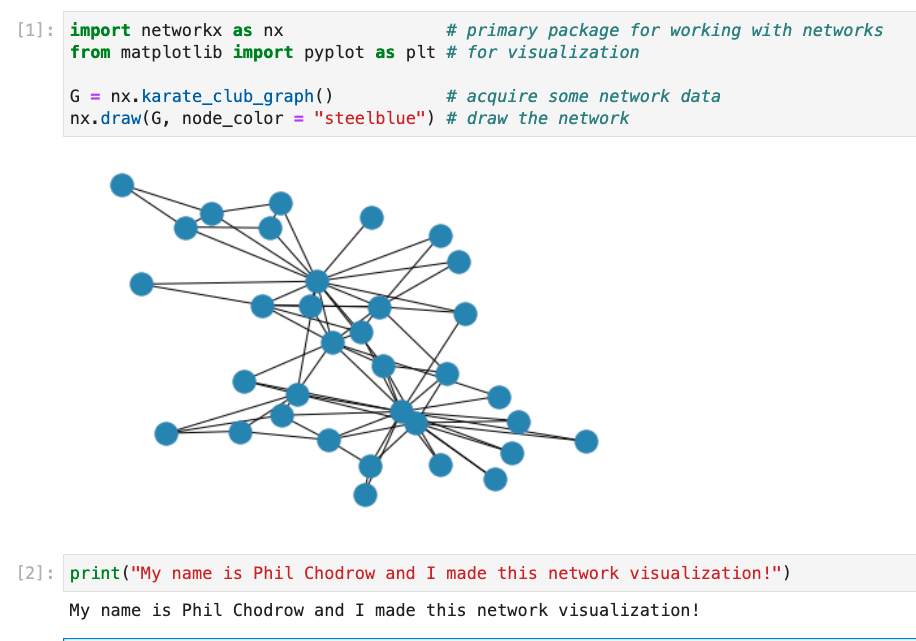
\includegraphics[width=\textwidth]{img/network-viz.png}


    

\problem{}

    In this problem, you will argue that a binomial distribution can be approximated by a Poisson distribution in a certain limit. 
    This approximation will be useful when we study properties of random graph models. 
    
    As a reminder, a nonnegative discrete random variable $X$ has a \emph{binomial distribution} with number of trials $n$ and success rate $p$ if its probability mass function is 
    \begin{align*}
        p_X(k) = \binom{n}{k}p^{k}(1-p)^{n-k}\;. 
    \end{align*}
    A nonnegative discrete random variable $Y$ has a \emph{Poisson distribution} with parameter $\mu$ if its probability mass function is 
    \begin{align*}
        p_Y(k) = \frac{\mu^ke^{-\mu}}{k!}\;. 
    \end{align*}
    Suppose now that $X$ is binomial and that $p = c / n$. 
    Show that, as $n$ grows large, $X$ is distributed approximately Poisson. 
    Identify the parameter of the Poisson distribution in terms of $c$ and $n$. 
    It suffices to show that the PMF of $X$ converges to a Poisson PMF (formally, we are showing \emph{convergence in distribution}). 

    An argument with calculations to back it up, rather than a formal proof, is sufficient. 
    You may need to find some useful approximations for quantities like $\binom{n}{k}$ and $e^m$. 
    You're welcome to use anything you can find, as long as you \textbf{cite your sources}. 

    


\problem{}



    Let $X_1,\ldots,X_n$ be $n$ independent random variables with finite variance. 
    Let $Y = \sum_{i = 1}^n X_i$. 

    \part 
    Prove formally that 
    \begin{align*}
        \mathrm{var}(Y) = \sum_{i = 1}^n \mathrm{var}(X_i)\;. 
    \end{align*}

    

    \part 

    Assume now that $X_1,\ldots,X_n$ are also identically distributed. 
    Let $y = \mathbb{E}[Y]$. 
    Using your result from the previous part, derive a bound on the probability that the \emph{absolute error} $\lvert Y - y\rvert$ is large.
    Formally, fill in the righthand side in the inequality 
    \begin{align*}
        \mathbb{P}(\lvert Y - y\rvert > \epsilon) < \; ???
    \end{align*}

    

    \part 

    Give a similar bound for the \emph{relative error}: using Part (a), fill in the righthand side in 

    \begin{align*}
        \mathbb{P}\left(\frac{\lvert Y - y\rvert}{\lvert y \rvert} > \epsilon\right) < \; ???
    \end{align*}


    

    \part 
    
    Comment briefly on what can be said about the absolute error as $n$ grows large. 
    What about the relative error? 
    
    




\end{document}